\RequirePackage[l2tabu, orthodox]{nag}

\documentclass{beamer}

\usepackage{microtype}
\usepackage{amsmath,amssymb}
%??? :( \usepackage[MnSymbol]{mathspec}
\usepackage{mathspec}
\usepackage[final]{listings}
\usepackage{graphicx}

\setallmainfonts{TeX Gyre Schola}
\setallmonofonts{Menlo}

%\usepackage{xunicode}
%\usepackage{xltxtra}
%\usepackage{graphicx}
%\usepackage{forloop}
%\usepackage{stmaryrd}
%\usepackage{mathtools}
%\usepackage{fancyvrb}

\usepackage{tikz}
% \usetikzlibrary{arrows.meta}
% \usetikzlibrary{backgrounds}
\usetikzlibrary{calc}
% \usetikzlibrary{datavisualization}
% \usetikzlibrary{datavisualization.formats.functions}
\usetikzlibrary{math}
% \usetikzlibrary{fit}
% \usetikzlibrary{positioning}
% \usetikzlibrary{scopes}
\usetikzlibrary{shapes.geometric}

\def\bigO#1{\ensuremath{\mathcal O(#1)}}
\def\BigO#1{\ensuremath{\mathcal O\left(#1\right)}}
\newcommand\fun[1]{\ensuremath{\lambda #1.\,}}
\renewcommand\T[1]{\ensuremath{T_{\mathit{#1}}}}

%%%
%%% BASIC SETTINGS
%%%

\frenchspacing
\unitlength=0.01\textwidth
\thicklines
\urlstyle{sf}
\graphicspath{{images/}}
\setlength{\parskip}{.25em}

\defaultfontfeatures{
    Mapping=tex-text,
    Scale=MatchLowercase,
}

%%%
%%% LISTINGS SETUP
%%%

\lstdefinelanguage{ASL}%
  {sensitive,%
   alsoletter=-+*/\#?,%
   alsodigit=-,%
   morekeywords={%
      and,%
      begin,%
      check-error,%
      check-expect,%
      check-within,%
      cond,%
      define,%
      define-struct,%
      else,%
      if,%
      lambda,%
      local,%
      or,%
   },%
   morekeywords=[2]{%
     cons,%
     \#true,%
     \#false,%
   },%
   morekeywords=[3]{%
     this-is-here-because-suck,%
     cons?,%
     empty?,%
     -,+,*,/,%
     first,%
     rest,%
   }%,
   morecomment=[l];,%
   morecomment=[s]{\#|}{|\#},%
   morestring=[b]"%
  }[keywords,comments,strings]%

\lstnewenvironment{ASL}[1][]
{%
  \begingroup
  \lstset{language=ASL,#1}%
}
{%
  \endgroup
}

\lstnewenvironment{CXX}[1][]
{%
  \begingroup
  \lstset{language=C++,#1}%
}
{%
  \endgroup
}

\lstnewenvironment{Java}[1][]
{%
  \begingroup
  \lstset{language=Java,#1}%
}
{%
  \endgroup
}

\lstnewenvironment{Python}[1][]
{%
  \begingroup
  \lstset{language=Python,#1}%
}
{%
  \endgroup
}


\lstnewenvironment{Ruby}[1][]
{%
  \begingroup
  \lstset{language=Ruby,#1}%
}
{%
  \endgroup
}

\newcommand{\textcode}{%
  \lstset{language=ASL,basicstyle=\ttfamily\small}%
  \lstinline
}

\lstset{%
  numberstyle=\scriptsize,
  showspaces=false,
  basicstyle=\ttfamily,
  keywordstyle=\ttfamily\color{red!70!black},
  keywordstyle=[2]\ttfamily\color{blue!70!black},
  keywordstyle=[3]\ttfamily\color{green!40!black},
  numberstyle=\ttfamily\color{blue!70!black},
  commentstyle=\itshape\color{violet!80!black},
  escapeinside={($}{$)},
}

\newcommand{\textasl}{%
  \lstset{language=ASL,basicstyle=\ttfamily\small}%
  \lstinline
}

\let\sup^

\catcode`\^\active\relax
\def^#1^{\textasl|#1|}

%%%
%%% BEAMER SETUP
%%%

\setbeamercolor{frametitle}{fg=black}
\setbeamercolor{normal text}{fg=black}

\usefonttheme{serif}

\setbeamertemplate{frametitle}
  {\begin{center}\medskip
   \insertframetitle\par
   \end{center}}

\setbeamertemplate{itemize item}{$\bullet$}

\setbeamertemplate{navigation symbols}{}
\setbeamertemplate{footline}[text line]{%
    \hfill\strut{%
        \small\color{black!75}%
        \texttt{\insertframenumber:\insertframeslidenumber}%
    }%
    \hfill%
}

\makeatletter
\newcount\frameslidetemp
\newcommand\insertframeslidenumber{%
  \frameslidetemp\c@page\relax
  \advance\frameslidetemp-\beamer@startpageofframe\relax
  \advance\frameslidetemp1\relax
  \the\frameslidetemp
}
\makeatother

%%%
%%% GENERALLY USEFUL LITTLE MACROS
%%%

% For using \alt within verbatim:
\newcommand\ALT[3]{\alt<#1>{#2}{#3}}

% Or: \ALT = \S\alt
\def\S#1#2{#2<#1>}

\newcommand<>\always[1]{#1}

\newcommand\widen[1][1.2]{%
    \setlength\baselineskip{#1\baselineskip}%
}

%%%
%%% COLORS
%%%

\newcommand\K[1]{\textcolor{orange!70!black}{#1}}
\newcommand\REF{\textcolor{green!50!black}{ref}}

%%%
%%% TIKZ
%%%

% \place[STYLE]{LOCATION}{CONTENT} places CONTENT at LOCATION, applying
% STYLE
\newcommand\place[3][]{%
  \tikz[orp] \node[#1] at (#2) {#3};%
}

% \anchor{NAME} creates an addressable TikZ coordinate at the current
% location.
\newcommand\anchor[1]{%
  \tikz[orp] \coordinate (#1);%
}

% \nil{NODE} draws a slash across the node; if NODE is a square then we
% get the standard graphic notation for null/nil.
\newcommand\nil[1][1em]{%
  \begin{tikzpicture}[nil]
    \node[pointer tail, line width=0, opacity=0] {};
    \draw[overlay]
      node[pointer tail] (dummy) {}
      (dummy.west |- dummy.south) -- (dummy.east |- dummy.north);
  \end{tikzpicture}%
}

\makeatletter
  \newcommand\cons[1][]{\cons@kont{#1}}
  \def\cons@kont#1#2(#3)#4#5{\struct@kont{#1}{}(#3){#4&#5}}

  \newcommand\struct[1][]{\struct@kont{#1}}
  \def\struct@kont#1#2(#3)#4{
      \node[draw, inner sep=0, #1] (#3) {%
        \begin{tabular}{|*{100}{c|}}
          \hline
          #4\\
          \hline
        \end{tabular}
      }
  }
\makeatother

% \genpointer[STYLE]{BEND}{TARGET}
\newcommand\genpointer[2][genpointer]{%
  \tikz[remember picture, #1]
    \draw
      node[pointer tail] {}
      edge[->, overlay] (#2) ;%
}

% \hpointer[BEND]{TARGET} for a highlighted pointer
\newcommand\hpointer[2][]{%
  \genpointer[highlit pointer,#1]{#2}%
}

% \ppointer[BEND]{TARGET} for a non-highlighted pointer
\newcommand\ppointer[2][]{%
  \genpointer[pointer,#1]{#2}%
}

% \pointer[BEND]{TARGET} is highlighted if used in a highlighted context
\newcommand\pointer[2][]{%
  \ifhighlit\let\pointertemp\hpointer\else\let\pointertemp\ppointer\fi
  \pointertemp[#1]{#2}%
}

\newcommand\genpointerbase[2][genpointer]{%
  \tikz[remember picture, #1]
    \draw node[pointer tail] (#2) {};%
}

\newcommand\ppointerbase[2][genpointer]{%
  \genpointerbase[pointer,#1]{#2}%
}

\newcommand\hpointerbase[2][genpointer]{%
  \genpointerbase[highlit pointer,#1]{#2}%
}

\newcommand\pointerbase[2][]{%
  \ifhighlit\let\pointertemp\hpointerbase\else\let\pointertemp\ppointerbase\fi
  \pointertemp[#1]{#2}%
}

\newcommand\genpointerpoint[3][genpointer]{
  \draw (#2) edge[->, remember picture, overlay, #1] (#3) ;
}

\newcommand\ppointerpoint[2][genpointer]{%
  \genpointerpoint[pointer,#1]{#2}%
}

\newcommand\hpointerpoint[2][genpointer]{%
  \genpointerpoint[highlit pointer,#1]{#2}%
}

\newcommand\pointerpoint[2][]{%
  \ifhighlit\let\pointertemp\hpointerpoint\else\let\pointertemp\ppointerpoint\fi
  \pointertemp[#1]{#2}%
}

\tikzset{
  onslide/.code args={<#1>#2}{%
    \only<#1>{\pgfkeysalso{#2}}
  },
  orp/.style={
    overlay,
    remember picture,
  },
  rem/.style={
    remember picture,
  },
  every node/.style={
    very thick,
    inner sep=3pt,
  },
  treenode/.style={
    circle,
    draw=black,
    inner sep=2pt,
  },
  subtree/.style={
    treenode,
    isosceles triangle,
    isosceles triangle apex angle=30,
    text width=1em,
    align=center,
    shape border rotate=90,
    anchor=apex,
    inner xsep=0pt,
    inner ysep=4pt,
    fill=orange!30!white,
    draw=orange!50!black,
  },
  balance/.style={
    draw=none,
    color=green!70!black,
    anchor=north,
  },
  bad balance/.style={
    balance,
    color=red,
    },
  every path/.style={very thick},
  ref/.style={
    draw=red,
    densely dotted,
    font=\ttfamily,
  },
  cons/.style={
    draw=black,
    font=\ttfamily,
  },
  genpointer/.style={
    solid,
    bend left=30,
    >=Latex,
  },
  pointer/.style={
    genpointer,
    color=blue!50!black,
    opacity=.5,
  },
  highlit pointer/.style={
    genpointer,
    color=red!70!black,
  },
  nil/.style={
    color=black!50,
  },
  pointer tail/.style={
    draw,
    circle,
    text width=0,
    text height=1ex,
    inner sep=0,
  },
  highlight base/.style={
    outer color=#1!50,
    inner color=#1!30,
  },
  highlight base/.default=yellow,
  highlight/.style={
    highlight base,
    color=yellow!50!white!90!black,
    draw opacity=0.5,
    thick,
    draw,
    rounded corners=2pt,
  },
  bintree/.style={
    level 1/.style={sibling distance=#1},
    level 2/.style={sibling distance=#1/2},
    level 3/.style={sibling distance=#1/4},
    level 4/.style={sibling distance=#1/8},
    level 5/.style={sibling distance=#1/16},
  },
  bintree/.default={8em},
}

\newif\ifhighlit
\highlitfalse

% \highlight<WHEN>[NAME]{CONTENT}
\newcommand<>\highlight[2][\relax]{%
  \ifx#1\relax
    \begin{tikzpicture}
  \else
    \begin{tikzpicture}[remember picture]
  \fi
    \node[
      inner sep=0pt,
      outer sep=0pt,
      text depth=0pt,
      align=left,
    ] (highlight temp) {%
        \only#3{\highlittrue}%
        #2%
        \only#3{\highlitfalse}%
    };
    \begin{scope}[on background layer]
      \coordinate (highlight temp 1) at
        ($(highlight temp.north east) + (2pt,2pt)$);
      \coordinate (highlight temp 2) at
        ($(highlight temp.base west) + (-2pt,-3pt)$);
      \node#3 [
        overlay,
        highlight,
        inner sep=0pt,
        fit=(highlight temp 1) (highlight temp 2),
      ] {};
    \end{scope}
    \ifx#1\relax
      \relax
    \else
      \node (#1) [
        overlay,
        inner sep=0pt,
        fit=(highlight temp 1) (highlight temp 2),
      ] {};
    \fi
  \end{tikzpicture}%
}

\newcommand\HI[2]{\highlight<#1>{#2}}

% \huncover[NAME]{STEP}{CONTENT} uncovers from STEP onward, highlighting
% at STEP but not thereafter.
\newcommand\huncover[3][\relax]{%
  \uncover<#2->{\highlight<#2>[#1]{#3}}%
}

% \huncover[NAME]{STEP}{CONTENT} onlys from STEP onward, highlighting
% at STEP but not thereafter.
\newcommand\honly[3][\relax]{%
  \only<#2->{\highlight<#2>[#1]{#3}}%
}

\begin{document}

%%%
%%% TITLE PAGE
%%%

\newcommand{\takeaways}{
  \begin{frame}{Take-aways}
    \begin{itemize}
      \item What’s a hash function? What makes a hash function good?
      \item What’s the purpose of a hash table? How does it work, and
        how can it “go wrong”?
      \item What’s the purpose of a Bloom filter? How does it work, and
        how can it “go wrong”?
      \item What does it mean for a data structure to be
        \emph{probabilistic}?
    \end{itemize}
  \end{frame}
}

\newcommand{\FN}[1]{\ensuremath{\mathop{\mathit{#1}}}}
\newcommand{\PrioQ}{\ensuremath{\mathsf{PrioQ}}}
\newcommand{\Element}{\ensuremath{\mathsf{Element}}}
\newcommand{\Bool}{\ensuremath{\mathsf{Bool}}}

\begin{frame}[fragile]\relax
  \thispagestyle{empty}

  %% Need to initialize Tikz opacity inside a frame, not outside:
  \begin{tikzpicture}[opacity=0,overlay]\end{tikzpicture}

  \begin{center}
    {\huge Probabilistic Data Structures}

  \bigskip
  \large
  EECS 214

  \medskip
  November 18, 2015
  \end{center}
\end{frame}

\takeaways

\begin{frame}[fragile]{Mappings}
  Remember counting byte frequencies in HW1?
  \par \pause \medskip
  You need(ed) a mapping from byte values to their counts:
  \[ \mathrm{byteFrequencies} : \{0, 1, \dotsc, 255\} \to \mathbb N \]
  How did you represent this?
  \par \pause \medskip
  Easy:
  \begin{CXX}
    size_t byte_freqs[256];
  \end{CXX}
  \pause
  \medskip
  Arrays are \emph{perfect} for mappings whose domain is $\{0, 1,
  \dotsc, k\}$ for some $k$
  \par\pause\medskip
  \emph{%
  Notation note: We will write $\mathbb N_k$ for the set $\{0, 1,
  \dotsc, k\}$
}
\end{frame}

\begin{frame}[fragile]{A different domain}
  What if we wanted to count word frequences instead?
  \par \pause \medskip
  We need a mapping from words (strings) to their counts:
  \[ \mathrm{wordFrequences} : \{ \text{ the set of all strings } \}
    \to \mathbb N \]
  How can we represent this?
  \par\pause\medskip
  We can't use strings to index into an array---we need a \emph{hash
  function}
\end{frame}

\begin{frame}{Definition: \emph{hash function}}
  A \emph{hash function} for some type maps values of
  that type to $\mathbb N_k$
  \par\pause\bigskip
  Here is a \textbf{really bad} hash function for strings:
  \[ \mathit{hash}_k(c_1\ldots c_n) = \sum_{i=1}\sup n \mathit{ord}(c_i)
  \quad \mathop{\mathrm{mod}} k \]
  \pause
  It adds up the character values
\end{frame}

\begin{frame}{How do we use a hash function?}
  A \emph{hash function} for some type maps values of that type to
  \alt<2>{indices into an array of size $k$}{$\mathbb N_k$}

  \uncover<3->{
    We then store our value $v$ at the index given by
    $\mathit{hash}(v)$.
  }
\end{frame}

\begin{frame}[fragile]{Example (using shitty string hash function)}
  Store word frequencies at the index given by the hash of the word:

  \begin{center}
    \begin{tikzpicture}[rem]
    \node[
      shape=ellipse,fill=yellow!80!white,minimum height=1.6in
    ] (hash) {$\mathit{hash}_7$};
    \node[anchor=west] at (1in,0) (output) {
      \begin{tabular}{|c|}
        \hline 0 \\
        \hline 0 \\
        \hline \alt<8->10 \\
        \hline \alt<7->10 \\
        \hline \alt<4->10 \\
        \hline 0 \\
        \hline 0 \\
        \hline
      \end{tabular}
    };
    \node[anchor=east] (input) at (-1in, 0) {
      \begin{minipage}{1.1in}
      \begin{overprint}
        \onslide<2-4>
        \hfill “^store^”
        \onslide<5-7>
        \hfill “^word^”
        \onslide<8>
        \hfill “^frequencies^”
        \onslide<9->
        \hfill “^at^”
      \end{overprint}
      \end{minipage}
    };
    \draw<3-4,6-7,8,9-> (input) edge[->] (hash);
    \draw<4> (hash) edge[->] node[above] {4} (output.230);
    \draw<7> (hash) edge[->] node[above] {3} (output.180);
    \draw<8> (hash) edge[->] node[above] {2} (output.130);
    \draw<9> (hash) edge[->] node[above] {\alert{3}} (output.180);
  \end{tikzpicture}
  \par\uncover<10>{\alert{Hash collision!}}
  \end{center}
\end{frame}

\begin{frame}[fragile]{Take two: separate chaining}
  Each bucket stores a linked list of associations:

  \begin{center}
    \begin{tikzpicture}[rem]
    \node[anchor=west] (output) {
      \begin{tabular}{|l|}
        \hline (hash, 1) \\
        \hline \\
        \hline (frequencies, 1) $\to$ (by, 1) \\
        \hline (word, 2) $\to$ (at, 1) $\to$ (of, 1) \\
        \hline (store, 1) $\to$ (index, 1) \\
        \hline (given, 1) \\
        \hline (the, 3) \\
        \hline
      \end{tabular}
    };
  \end{tikzpicture}
  \end{center}
  \par\pause
\end{frame}

\begin{frame}{Time complexity of hash table operations}
  What's the time complexity of insert? Lookup?
  \par\medskip\pause
  \emph{Depends on how many collisions we have!}
  \par\medskip\pause
  If we avoid collisions: \bigO{1} \emph{on average}
  \par\medskip\pause
  But too many collisions and the lists get too long: \bigO{n}
\end{frame}

\begin{frame}{Probabilities of collisions}
  \centering
  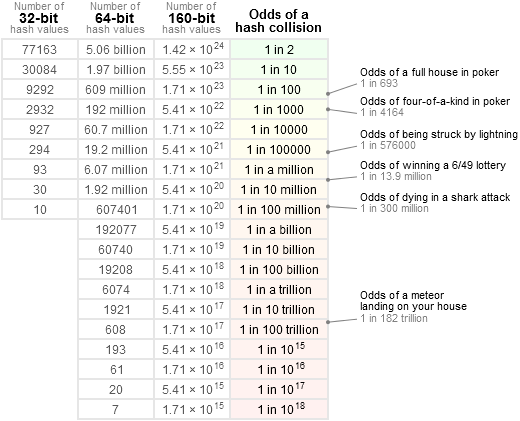
\includegraphics[width=3.5in]{probs.png}
\end{frame}

\begin{frame}{What makes a good hash function?}
  Inputs get scattered all over the range of the output
  \par\bigskip\pause
  Stronger: changing any one bit of the input changes each bit of the
  output with probability $\frac12$
\end{frame}

\takeaways

\end{document}
